%
% eindim.tex -- eindimensionales System mit optimaler Steuerung
%
% (c) 2024 Prof Dr Andreas Müller
%
\begin{figure}
\centering
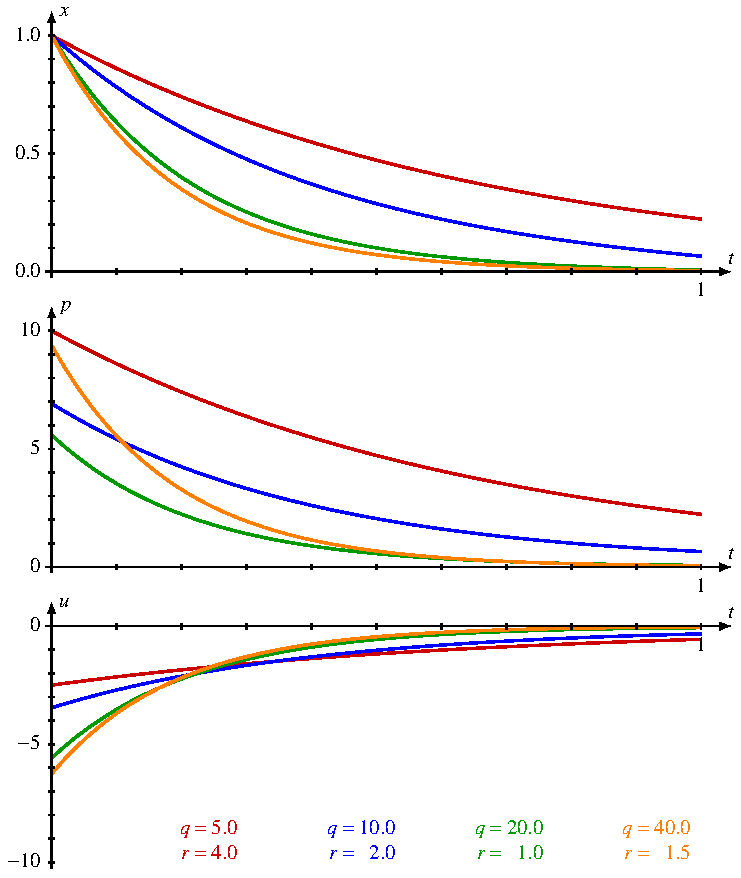
\includegraphics{chapters/080-hamiltonjacobi/examples/eindim.pdf}
\caption{Optimale Steuerung des Systems von Beispiel
\ref{buch:hamiltonjacobi:oc:bsp:eindim} für verschiedene Werte
der Gewichtungsfaktoren $q$ und $r$.
Der Faktor $s_1=10$, der die Abweichung von $0$ bewertet, wird nicht
verändert.
Grössere Werte von $q$ bedeuten grössere Kosten für eine Abweichung
des Zustands $x$ von $0$ und bewirken damit eine schneller Konvergenz.
Grosse Werte von $u$ haben die umgekehrte Wirkung: die Kosten der
Steuerung sind hoch, das System versucht die Konvergenz mit geringen
Steuereinflüssen zu erreichen.
\label{buch:hamiltonjacobi:fig:eindim}}
\end{figure}
